\documentclass{subfiles}

\begin{document}

    \chapter{Puesta en marcha y pruebas desarrolladas}
    \label{chap:puesta_en_marcha_y_pruebas_desarrolladas}

    \section{Alojamiento y ejecución}
    \label{sec:alojamiento_y_ejecucion}
    Para poder ejecutar la aplicación web desde cualquier dispositivo, fue necesario alojar el sistema en un servidor. Dado que la empresa \silverstorm era la primera interesada en el proyecto y ofrecía los recursos necesarios, permitió el uso de dos servidores de pequeña capacidad con sistema \linux proporcionado por \aws: uno para desarrollo y demostraciones internas y otro para su posterior uso en producción. Además, para poder cumplir los requisitos de \webxr, que requería del uso de conexiones seguras a través de HTTPS \cite{web:webxrrequirements}, era necesario utilizar certificados SSL. Esto se consiguió utilizando un certificado autofirmado para el entorno de desarrollo, y un certificado para la instancia de producción firmado por \textit{RapidSSL}, entidad utilizada para otras webs de la empresa.

    \paragraph{}
    Para alojar la aplicación en los servidores, se hizo uso de los comandos \textit{git} a través de la consola de \linux, de manera que se pudiese acceder siempre a la última versión del repositorio. Además, para asegurar que el contenido adecuado se traspasaba siempre al servidor correcto, se mantuvo la rama principal del repositorio como única rama a utilizar en el servidor de producción, siendo esto distinto en el servidor de desarrollo, donde se utilizaba la rama de desarrollo que estuviese activa en el momento, debido a que se creaban nuevas ramas para cada tarea. Una vez se descargaba el contenido en el servidor, mediante un script de \textit{Bash}, se movía el contenido descargado del repositorio para sobreescribir el antiguo contenido, que quedaba copiado en una carpeta aparte para ser recuperado en caso de problemas.

    \begin{figure}%[H]
    \centering
    \fbox{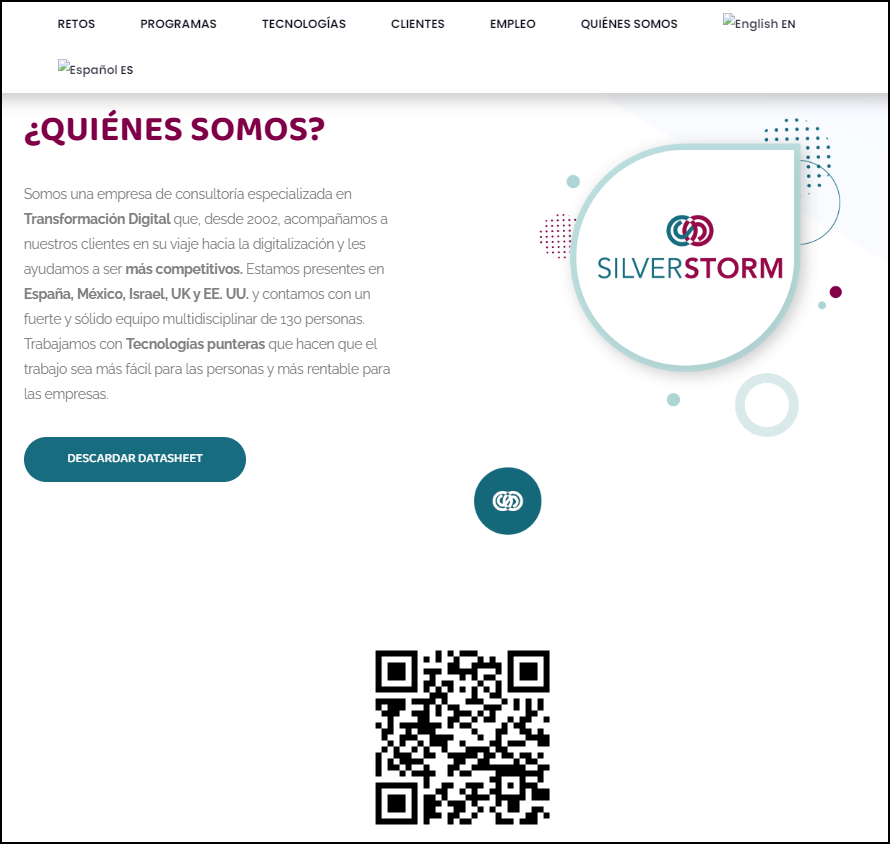
\includegraphics[width=0.5\textwidth]{img/5.1_qr_web.png}}
    \caption{El código QR insertado en la sección \textit{¿Quiénes somos?}.}
    \label{fig:5.1_qr_web}
    \end{figure}

    \paragraph{}
    Una vez estuvo configurado el servidor para alojar correctamente la aplicación, se comenzó el proceso para que el usuario pudiese acceder a esta. Este consistía en ubicar un código QR en la página web de \silverstorm que apuntase a la \textit{landing page} de la aplicación. Además, en caso de que el usuario accediese a la web desde un móvil, el QR también debía actuar como un hiperenlace, de manera que el usuario pudiese pulsar sobre este y acceder directamente a la aplicación de \ra. Para la generación del código QR, se utilizó la aplicación web gratuita \textit{QR Code Generator} \cite{web:qrcodegenerator}, sin embargo, debido a que es un proceso simple, actualmente existen múltiples plataformas capaces de hacer la misma tarea con resultados similares o incluso mejores de manera también gratuita.

    \paragraph{}
    La ubicación del código QR en la web fue sencillo, debido a que esta estaba creada a través de \wordpress. Sin embargo, es necesario mencionar que, debido a que la empresa fue posteriormente adquirida por \thirdera, esta web fue dada de baja, dado que todo el contenido importante sería migrado a sus webs, por lo que actualmente no se puede visitar el dominio.

    \paragraph{}
    Con el código QR instalado en la web, el procedimiento para iniciar la aplicación de \ra es muy sencillo: El usuario, navegando por la web desde su ordenador, vería el código QR. Este escanearía el código QR con el móvil, lo cual le redirigirá a la página principal de la aplicación, donde podrá pulsar el botón que carga la aplicación, continuando con el proceso que se comentó en el punto \ref{sec:funcionamiento_final_de_la_realidad_aumentada}. Si el usuario utilizara su móvil en lugar del ordenador para navegar por la web de la empresa, el camino sería muy similar: una vez llegue al código QR, pulsaría sobre este, lo cuál le redirigirá en el mismo navegador a la aplicación de \ra, pudiendo así pulsar sobre el botón e iniciar el proceso del punto \ref{sec:funcionamiento_final_de_la_realidad_aumentada}.

    \begin{figure}[H]
    \centering
    \fbox{
\includegraphics[width=0.25\textwidth]{img/5.1_qr_actualizado.png}}
    \caption{Código QR con la dirección URL de la aplicación web.}
    \label{fig:5.1_qr_actualizado}
    \end{figure}

    \section{Pruebas de campo}
    \label{sec:pruebas_de_campo}
    Tanto durante el desarrollo de la aplicación como después de ser terminado el despliegue de la misma, hubo pruebas continuas para comprobar su la calidad y controlar posibles problemas y mejoras. Uno de los grandes puntos de inflexión que se dieron desde el inicio fue la calidad de los resultados de \hittest, encontrando una gran variabilidad de la calidad de este en relación con el dispositivo utilizado y con el entorno.

    \paragraph{}
    Para revisar dicha variabilidad, se reprodujeron numerosas pruebas bajo distintas condiciones, siendo estas las más frecuentes:
    \begin{enumerate}
        \item Utilizando un Xiaomi Redmi Note 9 Pro, con una cámara de 64MP, en una habitación con iluminación natural moderada y sobre un suelo de baldosa, el sistema tarda aproximadamente 5 segundos en encontrar la superficie.
        \item Utilizando un Samsung Galaxy A10, con una cámara de 13MP, en una habitación con iluminación artificial alta y sobre un suelo laminado de madera, el sistema tarda aproximadamente 40 segundos en encontrar la superficie.
    \end{enumerate}

    A partir de las distintas pruebas bajo estas condiciones se encontró lo siguiente:

    \paragraph{}
    En primer lugar, se encontró que los dispositivos móviles con cámaras de mejor calidad eran los que mejores resultados obtenían del \hittest, presumiblemente por obtener imágenes con mejor definición de las superficies, lo que ayudaría al sistema a interpretar y calcular los planos que después tendría que representar. Los dispositivos con cámaras de menor calidad tardaban más en encontrar superficies o no las reconocían bien.

    \paragraph{}
    En segundo lugar, también se detectó que en las pruebas existían problemas inherentes al entorno. Por un lado, el material del que estuviese hecha la superficie podía generar problemas al sistema a la hora de interpretarlo debido a imperfecciones, reflejos o brillos. Esto se comprobó en suelos de baldosa donde, dependiendo del lugar, tenían diferente reflejo debido al desgaste: las zonas más desgastadas permitían al sistema calcular mejor la superficie, mientras que las que conservaban mejor el brillo y reflejaban más la luz hacían que el sistema tardase más en detectarlo. Esta diferencia llegaba a ser de 5 segundos aproximadamente en superficies <<fáciles>> a 2 minutos en los casos más generales en superficies <<difíciles>>. Esto venía a su vez afectado por la cantidad de luz en el ambiente, siendo lo óptimo una cantidad de luz moderada y, a poder ser, natural, debido a que esta iluminación tiende a ser más uniforme, aunque una luz artificial moderada también es favorable para esta aplicación. En los casos de luz escasa, el sistema interpreta mal las superficies o, directamente, no las encuentra, mientras que con una luz demasiado fuerte el sistema puede no ser capaz de encontrar ninguna superficie, dependiendo del material de esta.

    \paragraph{}
    Durante el proyecto se preparó un documento de pruebas utilizado para detallar cada aspecto a probar, dándose el producto final en el caso de que todos estos puntos fueran correctos. Estos puntos cubren, de manera general, todos los requisitos descritos inicialmente en el capítulo \ref{sec:analisis_de_requisitos}.

% \usepackage{color}
% \usepackage{tabularray}
\definecolor{Silver}{rgb}{0.752,0.752,0.752}
\begin{longtblr}[
  caption = {Plan de pruebas desarrollado.},
  label = {tab:plan_de_pruebas_desarrollado},
]{
  width = \linewidth,
  colspec = {Q[100]Q[170]Q[80]Q[294]Q[294]},
  row{1} = {Silver,c},
  cell{2}{1} = {r=4}{},
  cell{2}{2} = {r=4}{},
  cell{6}{1} = {r=3}{},
  cell{6}{2} = {r=3}{},
  cell{9}{1} = {r=2}{},
  cell{9}{2} = {r=2}{},
  vlines,
  hline{1-2,6,9,11-17} = {-}{},
  hline{3-5,7-8,10} = {3-5}{},
}
\textbf{Código} & \textbf{Nombre} & \textbf{Paso} & \textbf{Descripción del paso} & \textbf{Resultados esperados}\\
\textbf{FP0010} & Arranque de la animación desde Android & \textbf{S010} & Acceder a
  https://silver-storm.com desde un móvil con SO Android & Se abre la
  página web de Silver-Storm\\
 &  & \textbf{S020} & Seleccionar
  idioma español & Se cambia el
  idioma a español y aparece un código QR\\
 &  & \textbf{S030} & Pulsar
  sobre la imagen QR & Se abre una
  página nueva con un botón Start\\
 &  & \textbf{S040} & Pulsar sobre el
  botón Start & Se arranca la
  cámara del móvil con un puntero para posicionar el avatar\\
\textbf{FP0020} & Arranque de la animación desde un móvil no
  Android & \textbf{S010} & Acceder a
  https://silver-storm.com desde un móvil con SO no Android & Se abre la
  página web de Silver-Storm\\
 &  & \textbf{S020} & Seleccionar
  idioma español & Se cambia el
  idioma a español y aparece un código QR\\
 &  & \textbf{S030} & Pulsar
  sobre la imagen QR & Se abre una
  página nueva con un mensaje "Tu navegador no permite una sesión de
  Realidad Aumentada"\\
\textbf{FP0025} & Arranque de la animación mediante QR & \textbf{S010} & Acceder a
  https://silver-storm.com desde un ordenador & Se abre la
  página web de Silver-Storm\\
 &  & \textbf{S020} & Seleccionar
  idioma español & Se cambia el
  idioma a español y aparece un código QR\\
 &  & \textbf{S030} & Desde
  un móvil escanear el código QR & Si el móvil
  tiene SO Android se abre una página nueva con un botón Start y si no es
  Android con el mensaje "Tu navegador no permite una sesión de Realidad
  Aumentada"\\
\textbf{FP0030} & Carga
  de modelo 3D aleatorio & \textbf{S010} & Dado
  el Test FP0010, pulsar en una zona lisa y aparentemente alejada 2 ó 3 metros
  del usuario & Se
  posicionar un avatar humano que aleatoriamente pude ser un hombre o una mujer
  punto seleccionado con las proporciones de una persona posicionada a dicha
  distancia\\
\textbf{FP0040} & Posicionar y
  redimensionar el modelo & \textbf{S010} & Dado el Test
  FP0030, volver a pulsar sobre una zona situada a unos 4 ó 5 metros del
  usuario & El
  avatar se posiciona en el punto seleccionado cambiando la proporción al nuevo
  punto\\
\textbf{FP0050} & Animación del
  esqueleto & \textbf{S010} & Dado
  el Test FP0030 & El
  avatar inicia una secuencia de movimientos del esqueleto que va en
  consonancia con los puntos que explica el audio\\
\textbf{FP0060} & Animación de la
  boca & \textbf{S010} & Dado
  el Test FP050 & El
  avatar inicia una secuencia de movimientos de la boca similar a la
  pronunciación del audio\\
\textbf{FP0070} & Audio
  acompasado por los movimientos & \textbf{S010} & Dado
  el Test FP030 & Se
  inicia la locución grabada que va acompasada con los movimientos del cuerpo y
  de los labios
\end{longtblr}

    Todas las pruebas comentadas en esta tabla resultaron exitosas, hecho por el cual se pudo obtener el producto final, en relación a lo comentado anteriormente en esta misma sección. Además, al cubrir estas pruebas los requisitos funcionales descritos en la sección \ref{sec:analisis_de_requisitos} y, a su vez, los casos de uso definidos en la sección \ref{sec:casos_de_uso}, se confirma que la aplicación cumple con los puntos expuestos durante el análisis del proyecto.

    \section{Problemas y errores}
    \label{sec:problemas_y_errores}
    A lo largo del desarrollo de la aplicación, han ido surgiendo múltiples errores, algunos más fáciles y otro más difíciles de depurar. La depuración de estos errores resultó generalmente complicada debido a que la aplicación debe ser abierta siempre a través de móvil, lo que obliga a configurar el móvil y conectarlo a través de cable a un ordenador para poder utilizar la consola del navegador. Además, los errores de programación que se encontrasen dentro del bucle principal serían especialmente problemáticos, porque no existe forma perfecta de ver la información necesaria de manera sencilla.

    \paragraph{}
    Sin embargo, la mayoría de los problemas que más bloquearon el desarrollo de la aplicación no estaban relacionados con \textit{bugs} surgidos durante el proceso y se acercaban bastante a los riesgos analizados en la sección \ref{sec:gestion_de_riesgos}. Después de un análisis de los problemas, estos son los considerados como más graves:
    \begin{itemize}
        \item La documentación de la librería \threejs resulta, en la gran mayoría de casos, insuficiente o deficientemente explicada, tal y como se previó en el riesgo RSK6. Esto ha afectado múltiples veces al avance del desarrollo, debido a que hay objetos que pertenecen a la librería pero que no se explica qué representan o cómo funcionan. Un caso muy particular es la función de carga de modelos \gltf, que solo viene explicada a través de un ejemplo, pero no hay ningún detalle sobre los objetos que devuelve dicha función. La falta de detalles en esta documentación ha obligado a descubrir muchos aspectos de esta librería a base de ensayo y error o a través de foros no oficiales y de dudosa calidad en Internet.
        \item De manera similar, y también relacionado con el riesgo RSK6, la documentación de \resonanceaudio también ha resultado ser muy escasa, constando solo de una página con el objeto principal y una lista de atributos y funciones de esta con una descripción muy básica y sin detallar, obligando prácticamente a basarse en los ejemplos que añade la página para poder obtener información mínima útil.
        \item Un problema relacionado con el código y que requirió de amplia y constante depuración fue la compatibilidad entre \threejs y \resonanceaudio a través de los objetos de representación de posiciones en tres dimensiones. Cada librería utiliza su propio objeto de posición y requiere de sus propias conversiones, lo que obligó a buscar la forma de compatibilizarlo, pero la dificultad para depurar objetos que se encuentran en el bucle de procesado de imágenes y la escasez de documentación al respecto hizo que los pasos para hacer compatible la información de ambas librerías fuera extremadamente lenta. Dado que este problema hubiera sido más liviano de haber tenido más experiencia, este puede relacionarse con el riesgo RSK5.
        \item De nuevo relacionado con el riesgo RSK6, y a pesar de que \webxr sí cuenta con documentación fiable y muy extensa a través de la web de desarrolladores de \textit{Mozilla}, la explicación para lanzar un sistema básico por parte de la web oficial de Google resulta muy escasa en muchos aspectos, omitiendo información que puede ser crucial en desarrollos más complejos. Un ejemplo de esto es la totalmente inexistente explicación de cuándo se solicita la imagen a la cámara y cómo se envía al \textit{canvas} generado. Además, \textit{Google} dispone de varios tutoriales distintos para lanzar un sistema básico a través de \webxr donde se ve información distinta y, a veces, contradictoria, lo que tampoco ayudó a lanzar una primera versión de la aplicación.
    \end{itemize}

    En todos estos casos, la solución final fue desarrollos a base de ensayo y error apoyándose en blogs y webs de desarrolladores independientes de los que se podían extraer datos que podrían ser importantes, tal y como se planteó en el plan de contingencia del riesgo RSK6, a pesar de que el riesgo RSK5 planteaba incluir personal de apoyo.

\end{document}